\documentclass[12 pt, leqno]{article}
\usepackage{latexsym}
\usepackage{amsmath}
\usepackage{amsfonts}
\usepackage{fancyhdr}
\usepackage{graphicx}
\usepackage[margin=1in]{geometry}
\setlength\parindent{20pt}
\usepackage{setspace} 
\newcommand{\indep}{\rotatebox[origin=c]{90}{$\models$}}
\usepackage{hyperref}


\begin{document}

\title{XGBoost / Tree Based Models Notes}
\author{Siddhartha Basu}
\date{\today}
\maketitle
\tableofcontents

\section{Context}

These notes are largely a summary of the following page \href{https://xgboost.readthedocs.io/en/stable/tutorials/model.html}{link}, the XGBoost documentation's tutorial ``Introduction to Boosted Trees''. Before reading this documentation, my understanding of random forests and boosting was limited to the following:

\begin{itemize}
\item Random forests use bagging (bootstrap aggregation) to average the prediction of many decision trees. Each decision tree is trained on a different bootstrap sample of the original training set. Each tree is also trained on a different subset of the full feature set.
\item Boosting means upsampling training examples where your algorithm performed poorly in order to get better overall performance. It is an additive model, where you sum up predictions of many trees (starting from the equal weight one).
\item Tree based models are generally fragile. Adding a single training example can drastically change the model.
\end{itemize}

XGBoost appears to approximate gradient boosted regression trees, where you can have a regression tree approximate the gradient. The term `gradient boosting' originates from the paper `Greedy Function Approximation: A Gradient Boosting Machine' by Friedman. 

Elements of Statistical Learning has the following useful summary of Bagging:

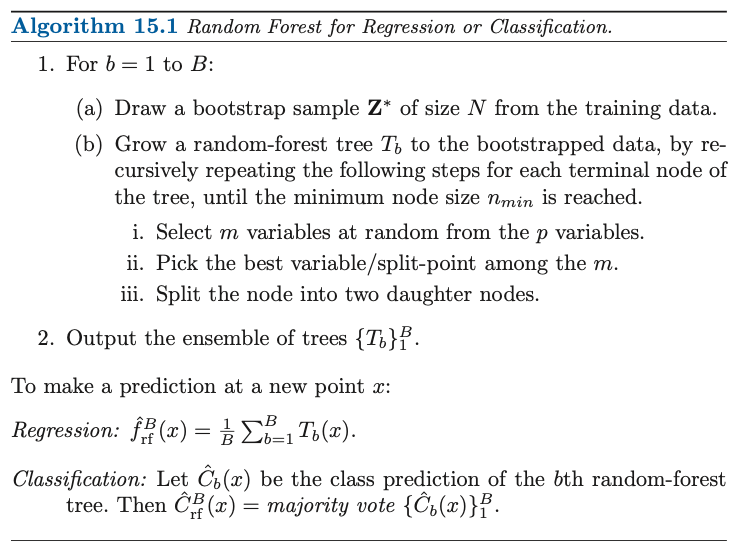
\includegraphics[scale=0.5]{bagging_esl}

Elements of Statistical Learning has the following summary of AdaBoost, a popular boosting algorithm as well. I think boosting is different from gradient boosting though. Gradient boosting re-defines boosting as a numerical optimization problem where the objective is to minimize the loss function of the model by adding weak learners using gradient descent. XGBoost uses stochastic gradient descent, randomly sampling observations and features in each step. 

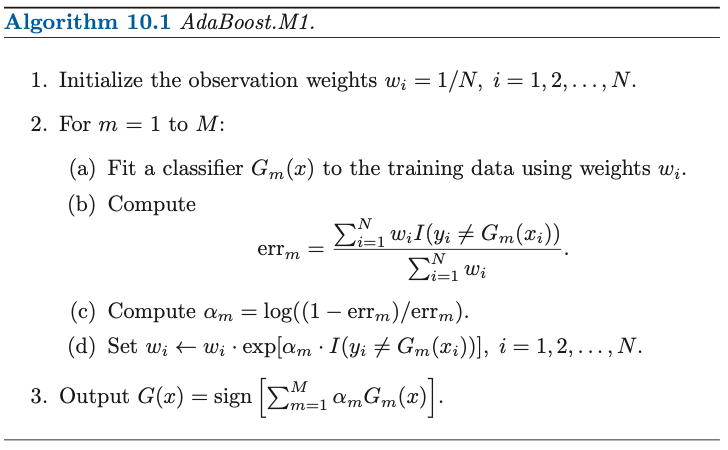
\includegraphics[scale=0.5]{boosting_esl}

\section{XGBoost documentation notes}
\subsection{Preliminaries from Supervised Learning}

The goal of training a model is to find the parameters $\theta$ that best fit the training data $x_i$ and labels $y_i$. The objective function generally has two parts, the training loss and the regularization term:

$$ \text{obj}({\theta}) = L(\theta) + \Omega(\theta) $$

Example choices of L include mean squared error:

$$L(\theta) = \sum_i (y_i - \hat{y}_i)^2$$

As well as logistic loss:

$$L(\theta) = \sum_i [ y_i \ln (1 + e^{-\hat{y}_i}) + (1 - y_i) \ln (1 + e^{\hat{y}_i}) ] $$

\subsection{Decision Tree Ensembles}

The model choice behind XGBoost is a decision tree ensemble. This model consists of a set of classification and regression trees (\textbf{CART}). A \textbf{decision tree} has leaves which contain decision values. In CART, a real score is associated with each leaf.

Let $\mathcal{F}$ be the set of all possible CART's, $K$ be the number of trees in your ensemble and $f_k$ be a function in the functional space $\mathcal{F}$. Then we can write the tree ensemble mathematically as:

$$\hat{y}_i = \sum_{k = 1}^{K} f_k(x_i)  \quad f_k \in \mathcal{F} $$

The objective function to be optimized over the $n$ training examples is given by:

$$ \text{obj}(\theta) = \sum_{i = 1} ^n l(y_i, \hat{y}_i) + \sum_{k = 1}^K \omega(f_k) $$

Where $\omega(f_k)$ is the complexity of tree $f_k$, which is defined later.

A visual representation of what is happening can be seen below:

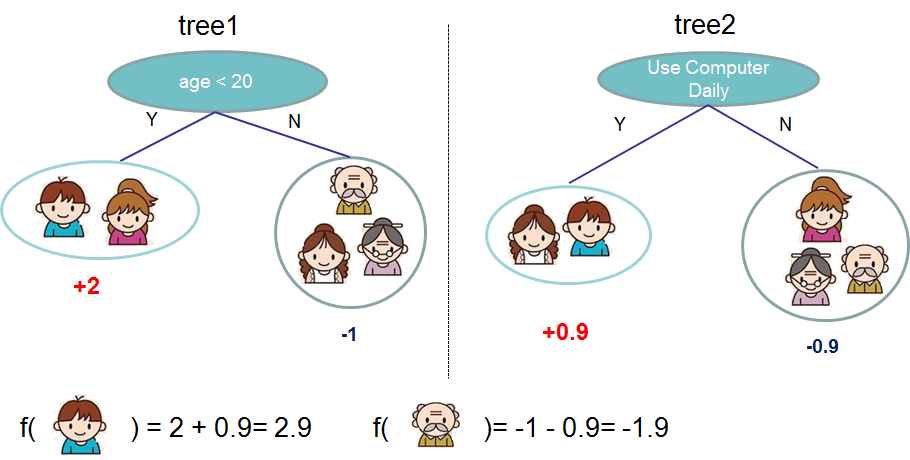
\includegraphics[scale=0.75]{tree_ensemble_example}

\subsection{Additive training}

Define the objective function to be the following:

$$ \text{obj}^{(t)} = \sum_{i = 1} ^n l(y_i, \hat{y}^{(t)}_i) + \sum_{i = 1}^t \omega(f_i)  $$

The general strategy for learning trees is additive, fix what we have learned and then add one new tree at a time. Let $\hat{y}^{(t)}_i$ be the prediction value at step t. Then the additive strategy is as follows:

\begin{align*}
\hat{y}^{(0)}_i &= 0 \\
\hat{y}^{(0)}_i &= f_1(x_i) = \hat{y}^{(0)}_i + f_1(x_i) \\
\hat{y}^{(2)}_i &= f_1(x_i) + f_2(x_i) = \hat{y}^{(1)}_i + f_2(x_i) \\
& \dots \\ 
\hat{y}^{(t)}_i &= \sum_{k = 1}^t f_k(x_i)  = \hat{y}^{(t - 1)}_i + f_t(x_i)
\end{align*}

The next question is, what tree do we want at each step? The natural choice would be to add the one that optimizes our objective. The goal is to find the tree $f_t$ that minimizes the following:

\begin{align*}
\text{obj}^{(t)} &= \sum_{i = 1} ^n l(y_i, \hat{y}^{(t)}_i) + \sum_{i = 1}^t \omega(f_i) \\ 
&= \sum_{i = 1} ^n l(y_i, \hat{y}^{(t-1)}_i + f_t(x_i)) + \omega(f_t) + \text{constant} 
\end{align*}

\subsubsection{Mean squared error loss}

If we use MSE as our loss function, our objective becomes:

\begin{align*}
\text{obj}^{(t)} &= \sum_{i = 1} ^n l(y_i, \hat{y}^{(t-1)}_i + f_t(x_i)) + \omega(f_t) + \text{constant} \\
&= \sum_{i = 1}^n [ 2(y_i^{(t-1)} - y_i) f_t (x_i) + f_t (x_i)^2 ] + \omega(f_t) + \text{constant}
\end{align*}

Where we expanded the quadratic, and then put the terms that only dealt with $y_i$ and $\hat{y}_i^{(t-1)}$ into the constant since they don't deal with the objective of optimization $f_t$.

\subsubsection{Taylor expansion}

In general, loss functions are not as friendly as MSE. In these cases we can take a second order Taylor expansion of the loss (I think with respect to $f_t$). The Taylor expansion of the loss is:

$$ \text{obj}^{(t)} = \sum_{i = 1}^n [l(y_i, \hat{y}_i^{(t - 1)}) + g_i f_t (x_i) + \frac{1}{2} h_i f_t^2 (x_i) ] + \omega(f_t) + \text{constant} $$

Here we have defined:

\begin{align*}
g_i &= \partial_{\hat{y}_i^{(t - 1)}} l(y_i, \hat{y}_i^{(t - 1)}) \\ 
h_i &= \partial^2_{\hat{y}_i^{(t - 1)}} l(y_i, \hat{y}_i^{(t - 1)})
\end{align*}

As the first and second derivatives of the objective with respect to the second input. After we remove the constants, the specific objective at step t becomes:

$$ \sum_{i = 1}^n [g_i f_t (x_i) + \frac{1}{2} h_i f_t^2 (x_i) ] + \omega(f_t) + \text{constant} $$

\subsection{Model complexity}

To complete the exposition of the training step, we now discuss the regularization term. First, we redefine the tree as:

$$f_t(x) = w_{q(x)} $$

Here, $w \in R^T$ is a vector of scores on every node. $q: R^d \rightarrow \{1, 2, \dots, T \}$ is a function assigning each training data point to a leaf. $T$ is the number of leaves in the tree. XGBoost defines the complexity as:

$$\omega(f) = \gamma T + \frac{1}{2} \lambda \sum_{j = 1}^T w_j^2 $$

\subsection{The Structure Score}

After redefining the tree as a vector of weights, we can reframe the optimization problem in terms of that vector. We can write the objective value with the $t$-th tree as:

\begin{align*}
\text{obj}^{(t)} &\approx \sum_{i = 1}^n [g_i w_{q(x_i)} + \frac{1}{2} h_i w^2_{q(x_i)} ] + \gamma T + \frac{1}{2} \lambda \sum_{j =1}^T w_j^2 \\
&= \sum_{j = 1}^T [(\sum_{i \in I_j} g_i) w_j + \frac{1}{2} (\sum_{i \in I_j} h_i + \lambda) w_j^2 ]  + \gamma T
\end{align*}

Here $I_j = \{i | q(x_i) = j \} $ us the set of indices of data points assigned to the $j$-th leaf. In the second line we have changed the index of the summation between the first and second line above. Initially we were summing over training examples $i$. Now we are summing over leafs in the tree $j$. We can do this because all data points on the same leaf get the same score $w_j$.

We can further compress the notation by defining $G_j = \sum_{i \in I_j} g_i$ and $H_j = \sum_{i \in I_j} h_i$. This allows us to write the objective as:

$$ \text{obj}^{(t)} = \sum_{j = 1}^T [G_j w_j + \frac{1}{2} (H_j + \lambda) w_j^2 ]  + \gamma T $$

This reveals the optimization as a relatively simple quadratic for each leaf in the tree. Given the tree structure, we can learn the best scores for each leaf in this way.

In this equation $w_j$ are independent with respect to each other, and the form $G_j w_j + \frac{1}{2} (H_j + \lambda) w_j^2$ is quadratic. The best $w_j$ for a given structure $q(x)$ and the best objective reduction we can get are:

\begin{align*}
w_j^* &= - \frac{G_j}{H_j + \lambda} \\ 
\text{obj}^* &= -\frac{1}{2} \sum_{j = 1}^T \frac{G_j^2}{H_j + \lambda} + \gamma T
\end{align*}

The following picture can explain this process. For a given tree structure, we can push the derivatives for each training example $g_i$ and $h_i$ to the leaves they belong to. Then we can sum the statistics together and use the formula to calculate how good the tree is.

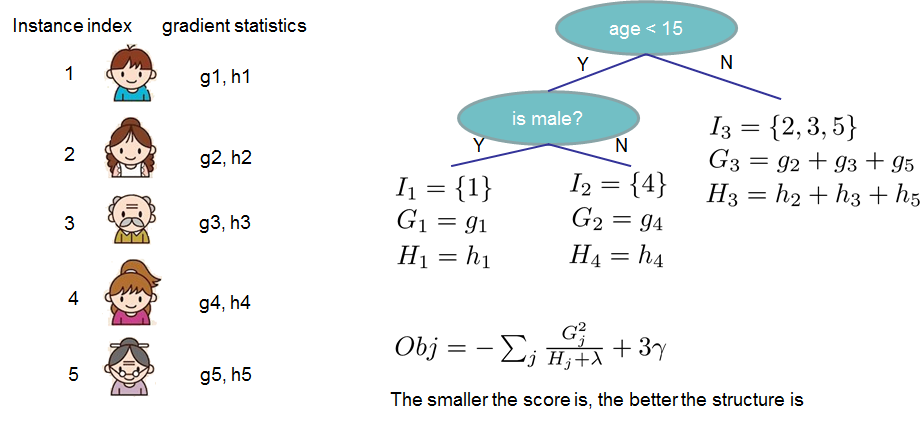
\includegraphics[scale=0.75]{struct_score}

\subsection{Learn the tree structure}

Finally, we can learn the tree structure by optimizing one level of the tree at a time. Specifically, we try to split a leaf into two leaves, we can check the score gain this split would achieve:

$$Gain = \frac{1}{2} \left( \frac{G_L^2}{H_L + \lambda} + \frac{G_R^2}{H_R + \lambda} - \frac{(G_L + G_R)^2}{H_L + H_R + \lambda} \right) - \gamma $$

The four terms that determine the gain are:

\begin{enumerate}
\item Add the score on the new left leaf
\item Add the score on the new right leaf
\item Subtract the score on the original leaf
\item Subtract the regularization penalty for adding a leaf
\end{enumerate}

If the gain in the objective is less than the regularization term, then you don't add the leaf split.

\section{Summary of XGBoost documentation}

The first key concept of gradient boosting is additive training, that we train several trees $f_k(x_i)$ that sum together to make a prediction:

$$\hat{y}_i^{(t)} = \sum_{k = 1}^t f_k(x_i) = \hat{y}_i^{(t-1)} + f_t(x_i)$$

We can plug this into a Taylor expansion of the loss/objective function that's centered at $l(y_i, \hat{y}_i^{(t-1)})$ and remove irrelevant terms in order to get the objective to be optimized at step $t$:

$$ \text{obj}^{(t)} = \sum_{i = 1}^n [g_i f_t (x_i) + \frac{1}{2} h_i f_t^2 (x_i) ] + \omega(f_t) + \text{constant} $$

We add in a regularization penalty of:

$$\omega(f) = \gamma T + \frac{1}{2} \lambda \sum_{j = 1}^T w_j^2 $$

Putting it all together, and changing the notation of the tree from $f_t(x_i)$ (an intractable function), to $w_{q(x)}$ a vector of scores on leaves ($q$ being the function assigning data points to leaves), we find the following objective function:

$$\text{obj}^{(t)} = \sum_{j = 1}^T [(\sum_{i \in I_j} g_i) w_j + \frac{1}{2} (\sum_{i \in I_j} h_i + \lambda) w_j^2 ]  + \gamma T $$

This is a relatively simple quadratic in $w_j$, and we can find the optimal scores and change to the objective:

\begin{align*}
w_j^* &= - \frac{G_j}{H_j + \lambda} \\ 
\text{obj}^* &= -\frac{1}{2} \sum_{j = 1}^T \frac{G_j^2}{H_j + \lambda} + \gamma T
\end{align*}

This gives us the optimal scores given a certain tree structure. To generate the optimal tree structure, we split leaves and calculate the score gain of the split, to see if it is worthwhile:

$$Gain = \frac{1}{2} \left( \frac{G_L^2}{H_L + \lambda} + \frac{G_R^2}{H_R + \lambda} - \frac{(G_L + G_R)^2}{H_L + H_R + \lambda} \right) - \gamma $$

\section{Bagging, Boosting and Gradient Boosting Blog Post Summary}

Summary of the following blog post: \href{https://towardsdatascience.com/bagging-boosting-and-gradient-boosting-1a8f135a5f4e}{link}

\subsection{Gradient Boosting}

Gradient boosting uses a gradient descent algorithm to minimize loss while adding models to the ensemble. Subsequent models are fit to pseudo residuals instead of adjusting weights. XGBoost also uses stochastic gradient descent, which adds randomness by sampling observations and features in each stage. This is similar to random forests, except this sampling is done without replacement. Gradient boosting looks for the optimal $h(x)$ where:

$$F_{m+1} (x) = F_m(x) + h(x) $$

The goal is to minimize the residual $y - F_m(x)$. The perfect $h$ would simply be:

$$h(x) = y - F_m(x)$$

The algorithm for gradient boosting is:

\begin{enumerate}
\item Initially, train on the dataset as normal and obtain predictions for each observation
\item Compute pseudo residuals as the negative of the partial derivative of the loss function with respect to the predictions from step 1.
\item Use pseudo residuals as new target for the next model and obtain predictions for each observation as before.
\item Repeat steps 2-3 for M iterations
\end{enumerate}

The pseudo residuals above are defined as:

$$r_{im} = - \left[ \frac{\partial L(y_i, F(x_i))}{\partial F(x_i)} \right]_{F(x) - F_{m-1} (x)} $$

In the XGBoost documentation, this appears equivalent to $g_i = \partial_{\hat{y}_i^{(t - 1)}} l(y_i, \hat{y}_i^{(t - 1)})$. The XGBoost documentation shows a two term Taylor expansion of the loss, and then an explanation of why going down the gradient (divided by the hessian) makes the most sense.

The blog post just says that we are reducing our approximation of the residual $y - F_m(x)$. The model becomes:

$$F_{m+1}(x) = F_m(x) - \partial_{F_m(x)} L(y, F_m(x)) $$ 

\textbf{Gradient Descent} works because a function's gradient is high in the directions that it changes a lot. 

\section{Open questions}

How do the different trees in the ``Additive training'' step / CART / decision ensembles relate to adding leafs in ``Learn the tree structure''. Jan 6 2023, it seems like each of the trees in the additive training step is one of the estimators in the \texttt{n estimators} hyperparameter when initiating an object in the XGBRegressor class. 

The XGBoost API reference \href{https://xgboost.readthedocs.io/en/stable/python/python_api.html}{link} defines \texttt{n estimators} as: Number of gradient boosted trees. Equivalent to number of boosting rounds.

How do random forests relate to the gradient boosting trees? They seem to be different. Further examination indicates that they are indeed different.






























































\end{document}